%%%%%%%%%%%%%%%%%%%%%%%%%%%%%%%%%%%%%%%%%
% Beamer Presentation
% LaTeX Template
% Version 1.0 (10/11/12)
%
% This template has been downloaded from:
% http://www.LaTeXTemplates.com
%
% License:
% CC BY-NC-SA 3.0 (http://creativecommons.org/licenses/by-nc-sa/3.0/)
%
%%%%%%%%%%%%%%%%%%%%%%%%%%%%%%%%%%%%%%%%%

%----------------------------------------------------------------------------------------
%	PACKAGES AND THEMES
%----------------------------------------------------------------------------------------

\documentclass{beamer}

\mode<presentation> {

% The Beamer class comes with a number of default slide themes
% which change the colors and layouts of slides. Below this is a list
% of all the themes, uncomment each in turn to see what they look like.

%\usetheme{default}
%\usetheme{AnnArbor}
%\usetheme{Antibes}
%\usetheme{Bergen}
%\usetheme{Berkeley}
%\usetheme{Berlin}
%\usetheme{Boadilla}
%\usetheme{CambridgeUS}
%\usetheme{Copenhagen}
%\usetheme{Darmstadt}
%\usetheme{Dresden}
\usetheme{Frankfurt}
%\usetheme{Goettingen}
%\usetheme{Hannover}
%\usetheme{Ilmenau}
%\usetheme{JuanLesPins}
%\usetheme{Luebeck}
%\usetheme{Madrid}
%\usetheme{Malmoe}
%\usetheme{Marburg}
%\usetheme{Montpellier}
%\usetheme{PaloAlto}
%\usetheme{Pittsburgh}
%\usetheme{Rochester}
%\usetheme{Singapore}
%\usetheme{Szeged}
%\usetheme{Warsaw}

% As well as themes, the Beamer class has a number of color themes
% for any slide theme. Uncomment each of these in turn to see how it
% changes the colors of your current slide theme.

%\usecolortheme{albatross}
%\usecolortheme{beaver}
%\usecolortheme{beetle}
%\usecolortheme{crane}
%\usecolortheme{dolphin}
%\usecolortheme{dove}
%\usecolortheme{fly}
%\usecolortheme{lily}
%\usecolortheme{orchid}
%\usecolortheme{rose}
%\usecolortheme{seagull}
%\usecolortheme{seahorse}
%\usecolortheme{whale}
%\usecolortheme{wolverine}

%\setbeamertemplate{footline} % To remove the footer line in all slides uncomment this line
%\setbeamertemplate{footline}[page number] % To replace the footer line in all slides with a simple slide count uncomment this line

%\setbeamertemplate{navigation symbols}{} % To remove the navigation symbols from the bottom of all slides uncomment this line
}

\usepackage{graphicx} % Allows including images
\usepackage{booktabs} % Allows the use of \toprule, \midrule and \bottomrule in tables
\usepackage{color}


%----------------------------------------------------------------------------------------
%	TITLE PAGE
%----------------------------------------------------------------------------------------

\title[OCC for Hop-HDFS]{Optimistic Concurrency Control in a Distributed NameNode Architecture for Hadoop Distributed File System} % The short title appears at the bottom of every slide, the full title is only on the title page

\author{Qi Qi} % Your name
\institute[IST/KTH/SICS] % Your institution as it will appear on the bottom of every slide, may be shorthand to save space
{
Instituto Superior T\'{e}cnico - IST (Portugal) \\ Royal Institute of Technology - KTH (Sweden) \\ 
Swedish Institute of Computer Science - SICS (Sweden) \\% Your institution for the title page
\medskip
\textit{qiq@kth.se} % Your email address
}
\date{19 September 2014} % Date, can be changed to a custom date

\begin{document}

\begin{frame}
\titlepage % Print the title page as the first slide
\end{frame}

\begin{frame}
\frametitle{Overview} % Table of contents slide, comment this block out to remove it
\tableofcontents % Throughout your presentation, if you choose to use \section{} and \subsection{} commands, these will automatically be printed on this slide as an overview of your presentation
\end{frame}

%----------------------------------------------------------------------------------------
%	PRESENTATION SLIDES
%----------------------------------------------------------------------------------------

%------------------------------------------------
\section{Introduction} % Sections can be created in order to organize your presentation into discrete blocks, all sections and subsections are automatically printed in the table of contents as an overview of the talk
%------------------------------------------------

\subsection{Motivation} % A subsection can be created just before a set of slides with a common theme to further break down your presentation into chunks

\begin{frame}
\frametitle{Motivation}
\begin{block}{Industrial Standard in Big Data Era}
	Apache Hadoop Ecosystem
\end{block}

\begin{block}{Limits to growth in HDFS}
	\begin{table}[ht]
		\centering
		\begin{tabular}{|c|c|c|}
			\hline
			\textbf{Number of Files} & \textbf{Memory Requirement} & \textbf{Physical Storage} \\ \hline
			1 million       & 0.6 GB             & 0.6 PB           \\ \hline
			{\color{red}\textbf{100 million}}     & {\color{red}\textbf{60 GB}}              & {\color{red}\textbf{60 PB}}            \\ \hline
			1 billion       & 600 GB             & 600 PB           \\ \hline
		\end{tabular}
	\end{table}
\end{block}

\begin{block}{Hop-HDFS and Its Limitation}
	Distributed NameNode Architecture \\ Restricted Concurrency
\end{block}
\end{frame}

%------------------------------------------------
\subsection{Problem Statement}
\begin{frame}
\frametitle{Problem Statement}
\begin{block}{HDFS}
	System-level Lock
\end{block}
\begin{block}{Hop-HDFS v1}
	System-level Lock
\end{block}
\begin{block}{Hop-HDFS v2}
	Row-level Lock
\end{block}
\begin{block}{MySQL Cluster}
	Read Committed / Anomalies
\end{block}
\end{frame}

%------------------------------------------------
\subsection{Contribution}
\begin{frame}
\frametitle{Contribution}
\begin{block}{Architectures and Namespace Concurrency Control}
GFS, HDFS, Hop-HDFS and MySQL Cluster
\end{block}

\begin{block}{Performance Accessment and Limitation Analysis}
HDFS v.s. Hop-HDFS v2 (PCC version)
\end{block}

\begin{block}{Solution for Hop-HDFS}
Optimistic Concurrency Control with Snapshot Isolation on Semantic Related Group
\end{block}
\end{frame}

%------------------------------------------------
\section{Background}

\subsection{GFS Architecture}
\begin{frame}
\frametitle{GFS Architecture}
\begin{figure}[h]
	\centering
	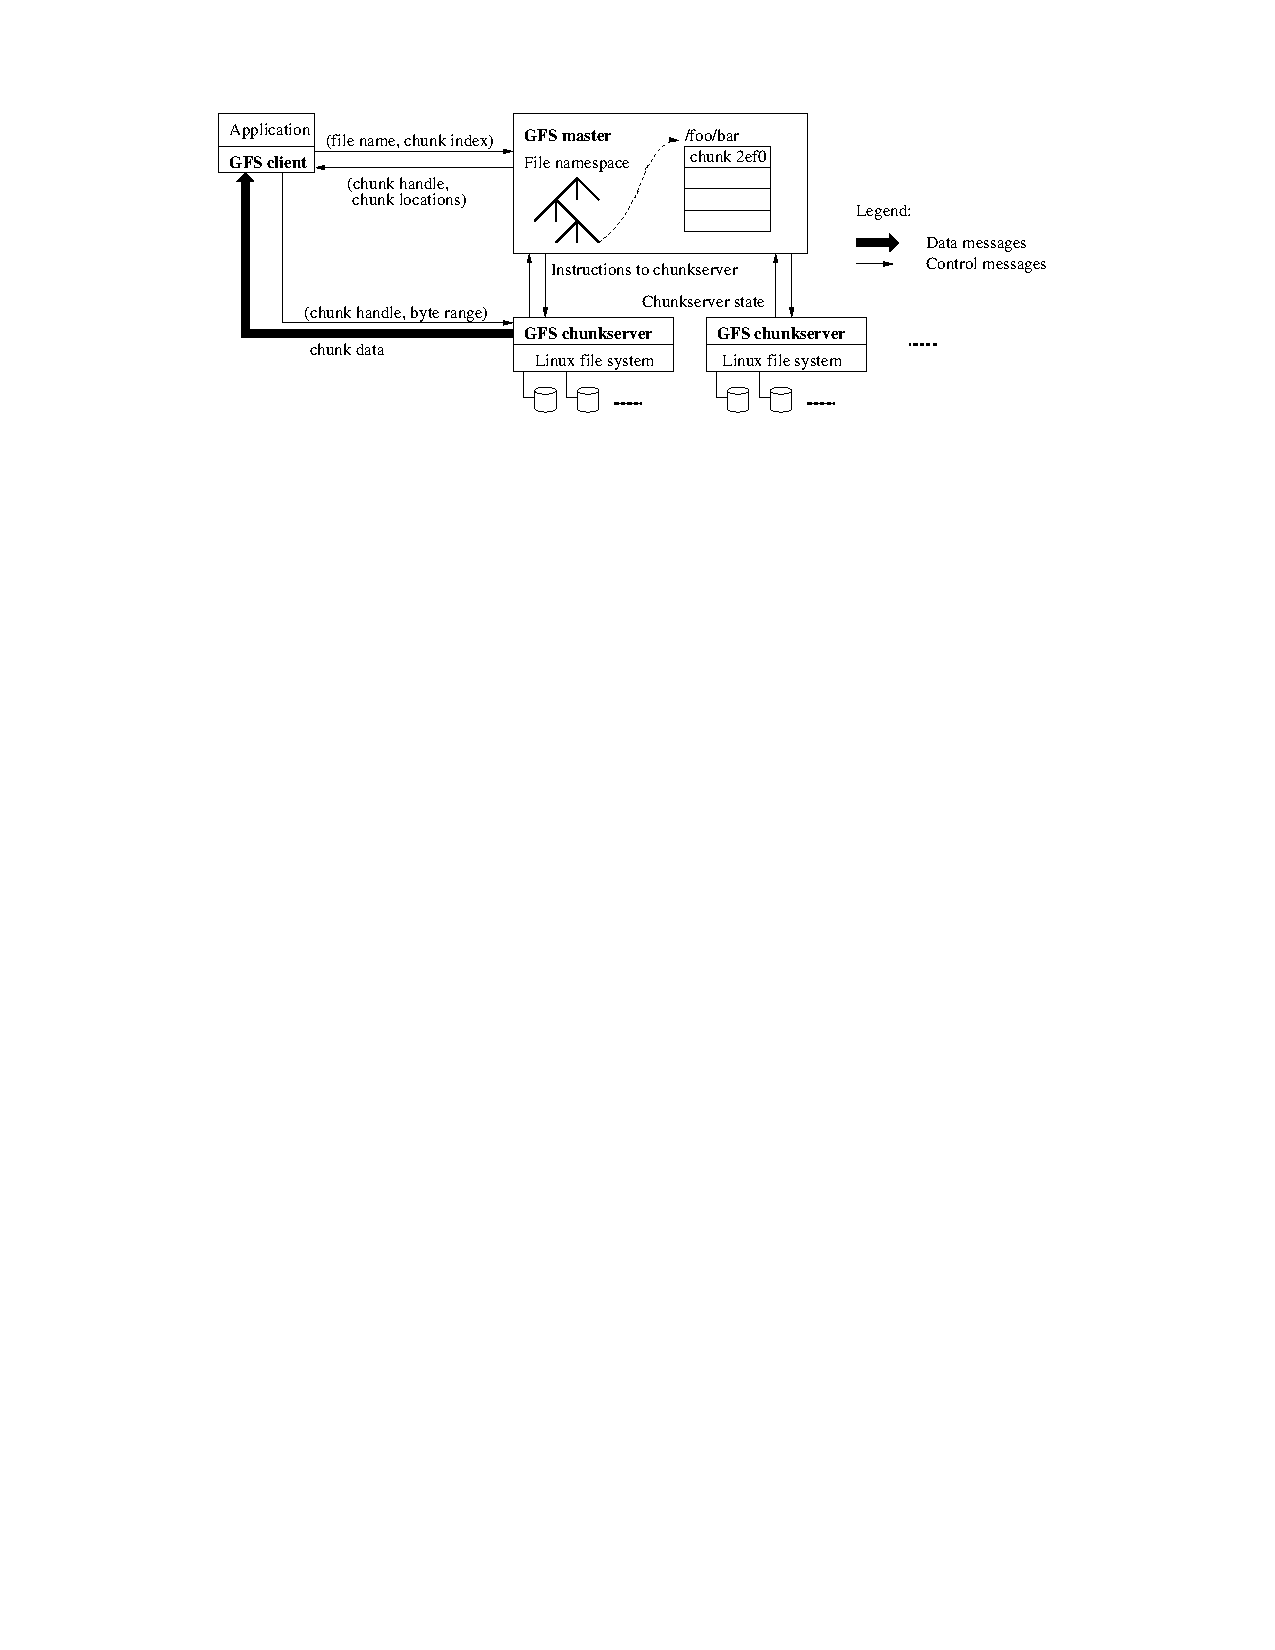
\includegraphics[width=\linewidth]{figs/GFSArchitecture.pdf}
\end{figure}
%\begin{columns}[c] % The "c" option specifies centered vertical alignment while the "t" option is used for top vertical alignment
%
%\column{.45\textwidth} % Left column and width
%\textbf{Heading}
%\begin{enumerate}
%\item Statement
%\item Explanation
%\item Example
%\end{enumerate}
%
%\column{.5\textwidth} % Right column and width
%Lorem ipsum dolor sit amet, consectetur adipiscing elit. Integer lectus nisl, ultricies in feugiat rutrum, porttitor sit amet augue. Aliquam ut tortor mauris. Sed volutpat ante purus, quis accumsan dolor.
%
%\end{columns}
\end{frame}

\subsection{HDFS Architecture}
\begin{frame}
	\frametitle{HDFS Architecture}
	\begin{figure}[h]
		\centering
		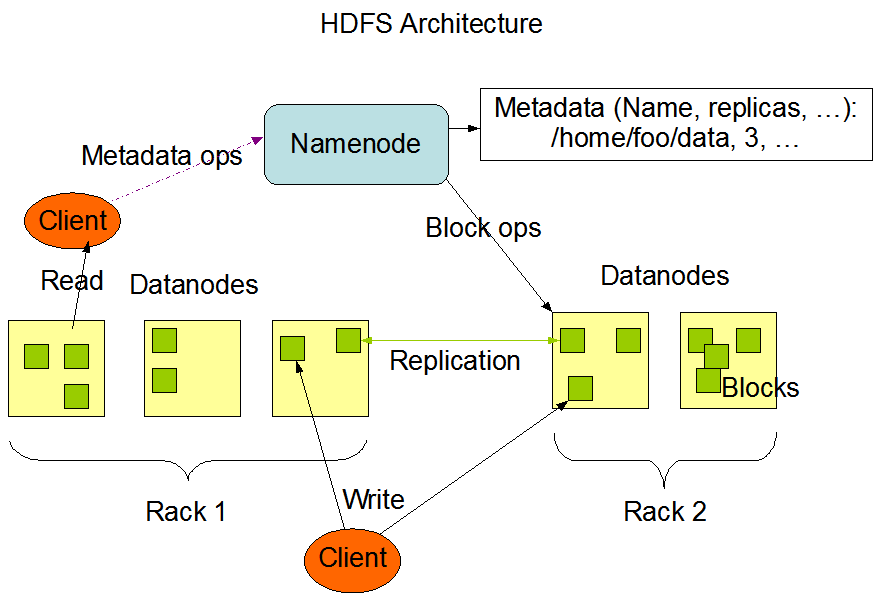
\includegraphics[width=\linewidth]{figs/hdfsarchitecturev1.png}
	\end{figure}
\end{frame}

\subsection{Isolation Level}
\begin{frame}
	\frametitle{Isolation Level}
	Berenson, Hal, et al. "A Critique of ANSI SQL Isolation Levels." ACM SIGMOD Record 24.2 (1995): 1-10.
\begin{table}[h]
	\centering
	\begin{tabular}{|c|p{1cm}|p{1cm}|p{1.5cm}|p{1cm}|p{1cm}|p{2cm}|p{1cm}|p{1cm}|}
		\hline
		\textbf{Isolation Level} &  \textbf{Lost Update} & \textbf{Fuzzy Read} & \textbf{Phantom} & \textbf{Read Skew} & \textbf{Write Skew} \\ \hline
		Read Uncommitted         &  \checkmark           & \checkmark          & \checkmark       & \checkmark         & \checkmark          \\ \hline
		Read Committed           &  \checkmark           & \checkmark          & \checkmark       & \checkmark         & \checkmark          \\ \hline
		Cursor Stability         &  some- times            & some- times           & \checkmark       & \checkmark         & some- times           \\ \hline
		Repeatable Read          & X                    & X                   & \checkmark       & X                  & X                   \\ \hline
		\textbf{Snapshot}                 & X                    & X                   & sometimes        & X                  & \checkmark          \\ \hline
		Serializable             & X                    & X                   & X                & X                  & X                   \\ \hline
	\end{tabular}
\end{table}
\end{frame}

\subsection{MySQL Cluster}
\begin{frame}
	\frametitle{MySQL Cluster}
	\begin{itemize}
		\item Distributed, in-memory, replicated database
		\item Supports only \textbf{Read Committed}
		\item High throughput:
	\end{itemize}
\begin{figure}[h!]
	\centering
	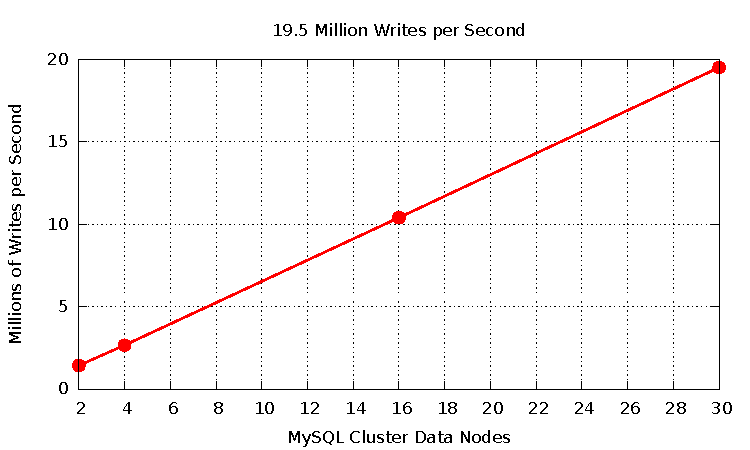
\includegraphics[scale=0.7]{figs/mysqlclusterbenchmark.pdf}
\end{figure}
\end{frame}

\subsection{Hop-HDFS}
\begin{frame}
	\frametitle{Hop-HDFS}
		\begin{block}{Overcome Limitations in HDFS NameNode}
			\begin{itemize}
				\item Scalability of the Namespace  
				\item Throughput Problem
				\item Failure Recovery
			\end{itemize}
		\end{block}
\end{frame}

\begin{frame}
	\frametitle{Hop-HDFS Architecture}
	\begin{figure}[h!]
		\centering
		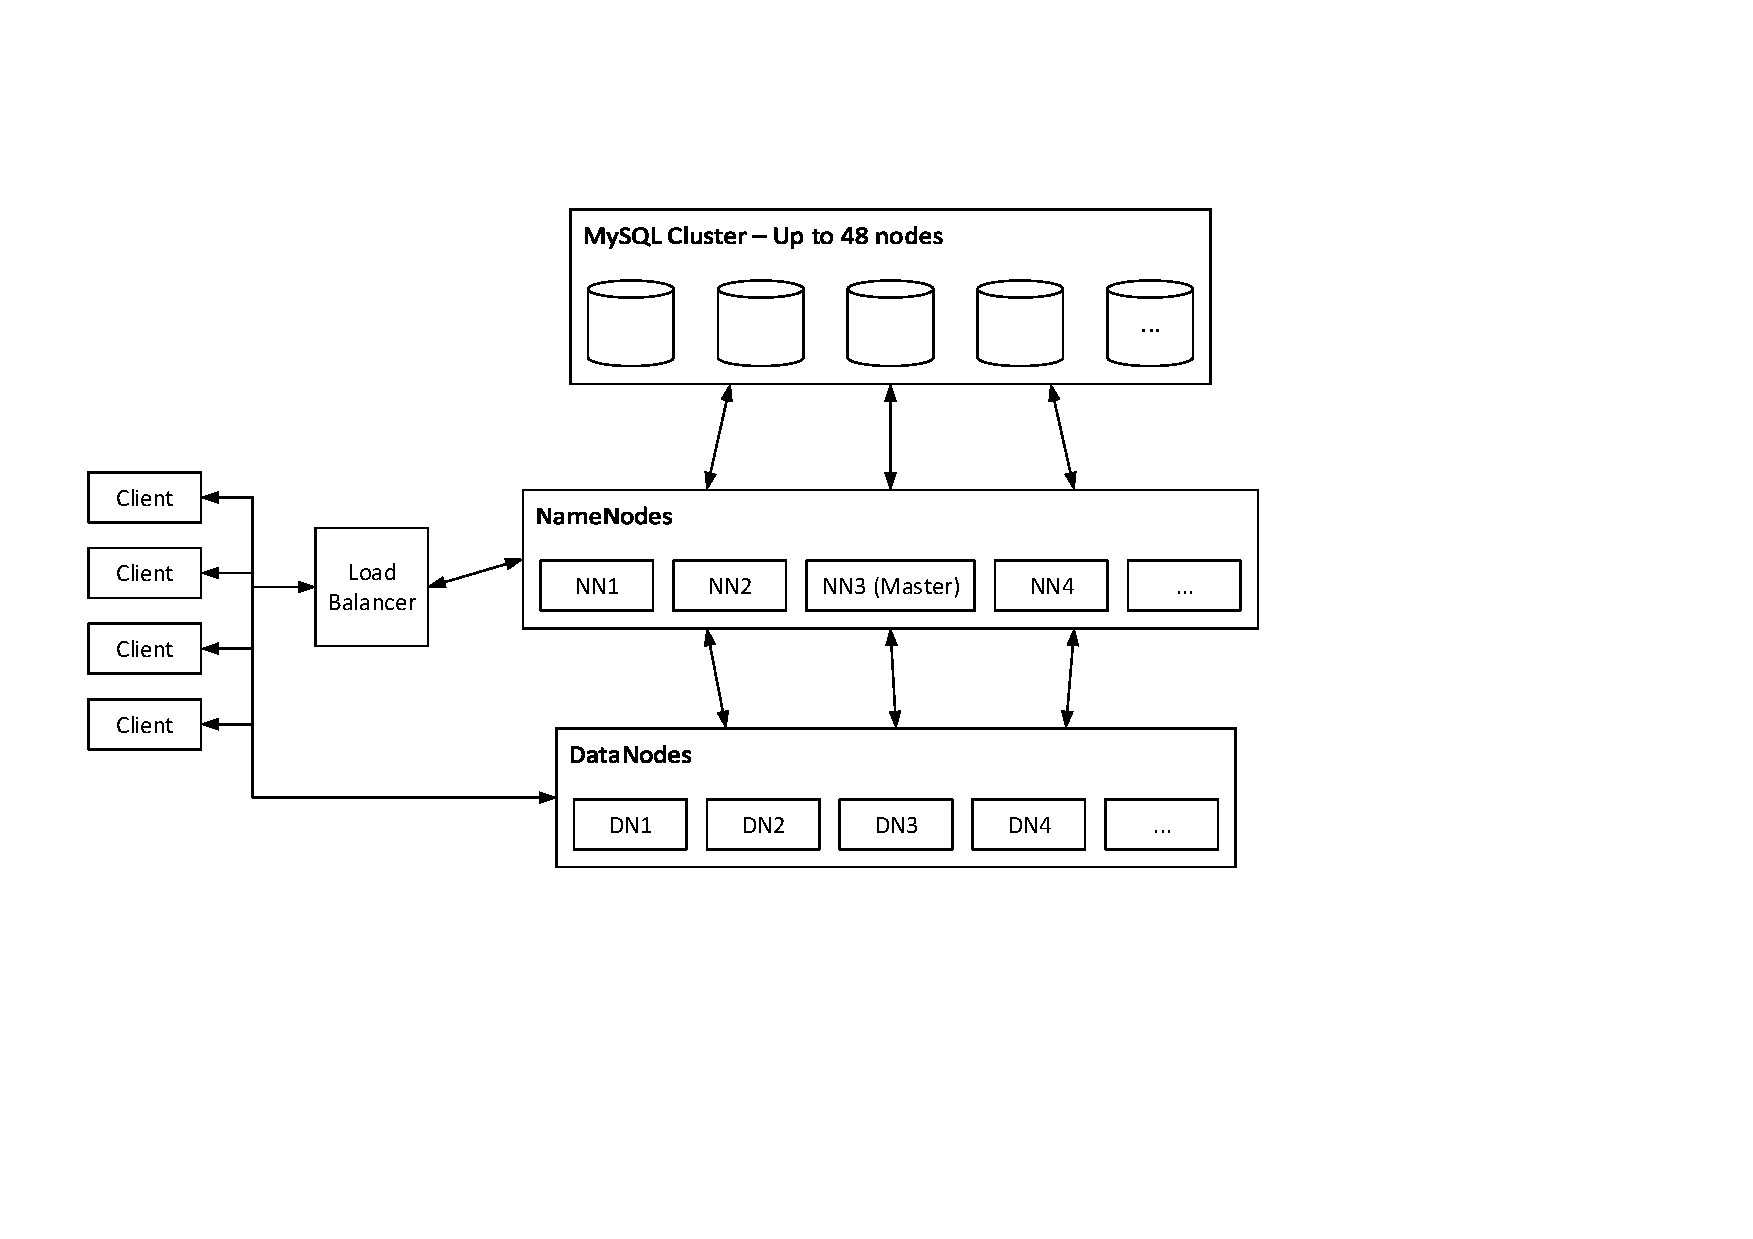
\includegraphics[width=\linewidth]{figs/HopHDFSArchitecture.pdf}
	\end{figure}
\end{frame}
%------------------------------------------------
\section{Namespace Concurrency Control}
%------------------------------------------------

\subsection{HDFS Namespace Concurrency Control}
\begin{frame}
	\frametitle{HDFS Namespace Concurrency Control}
		\begin{figure}[h]
			\centering
			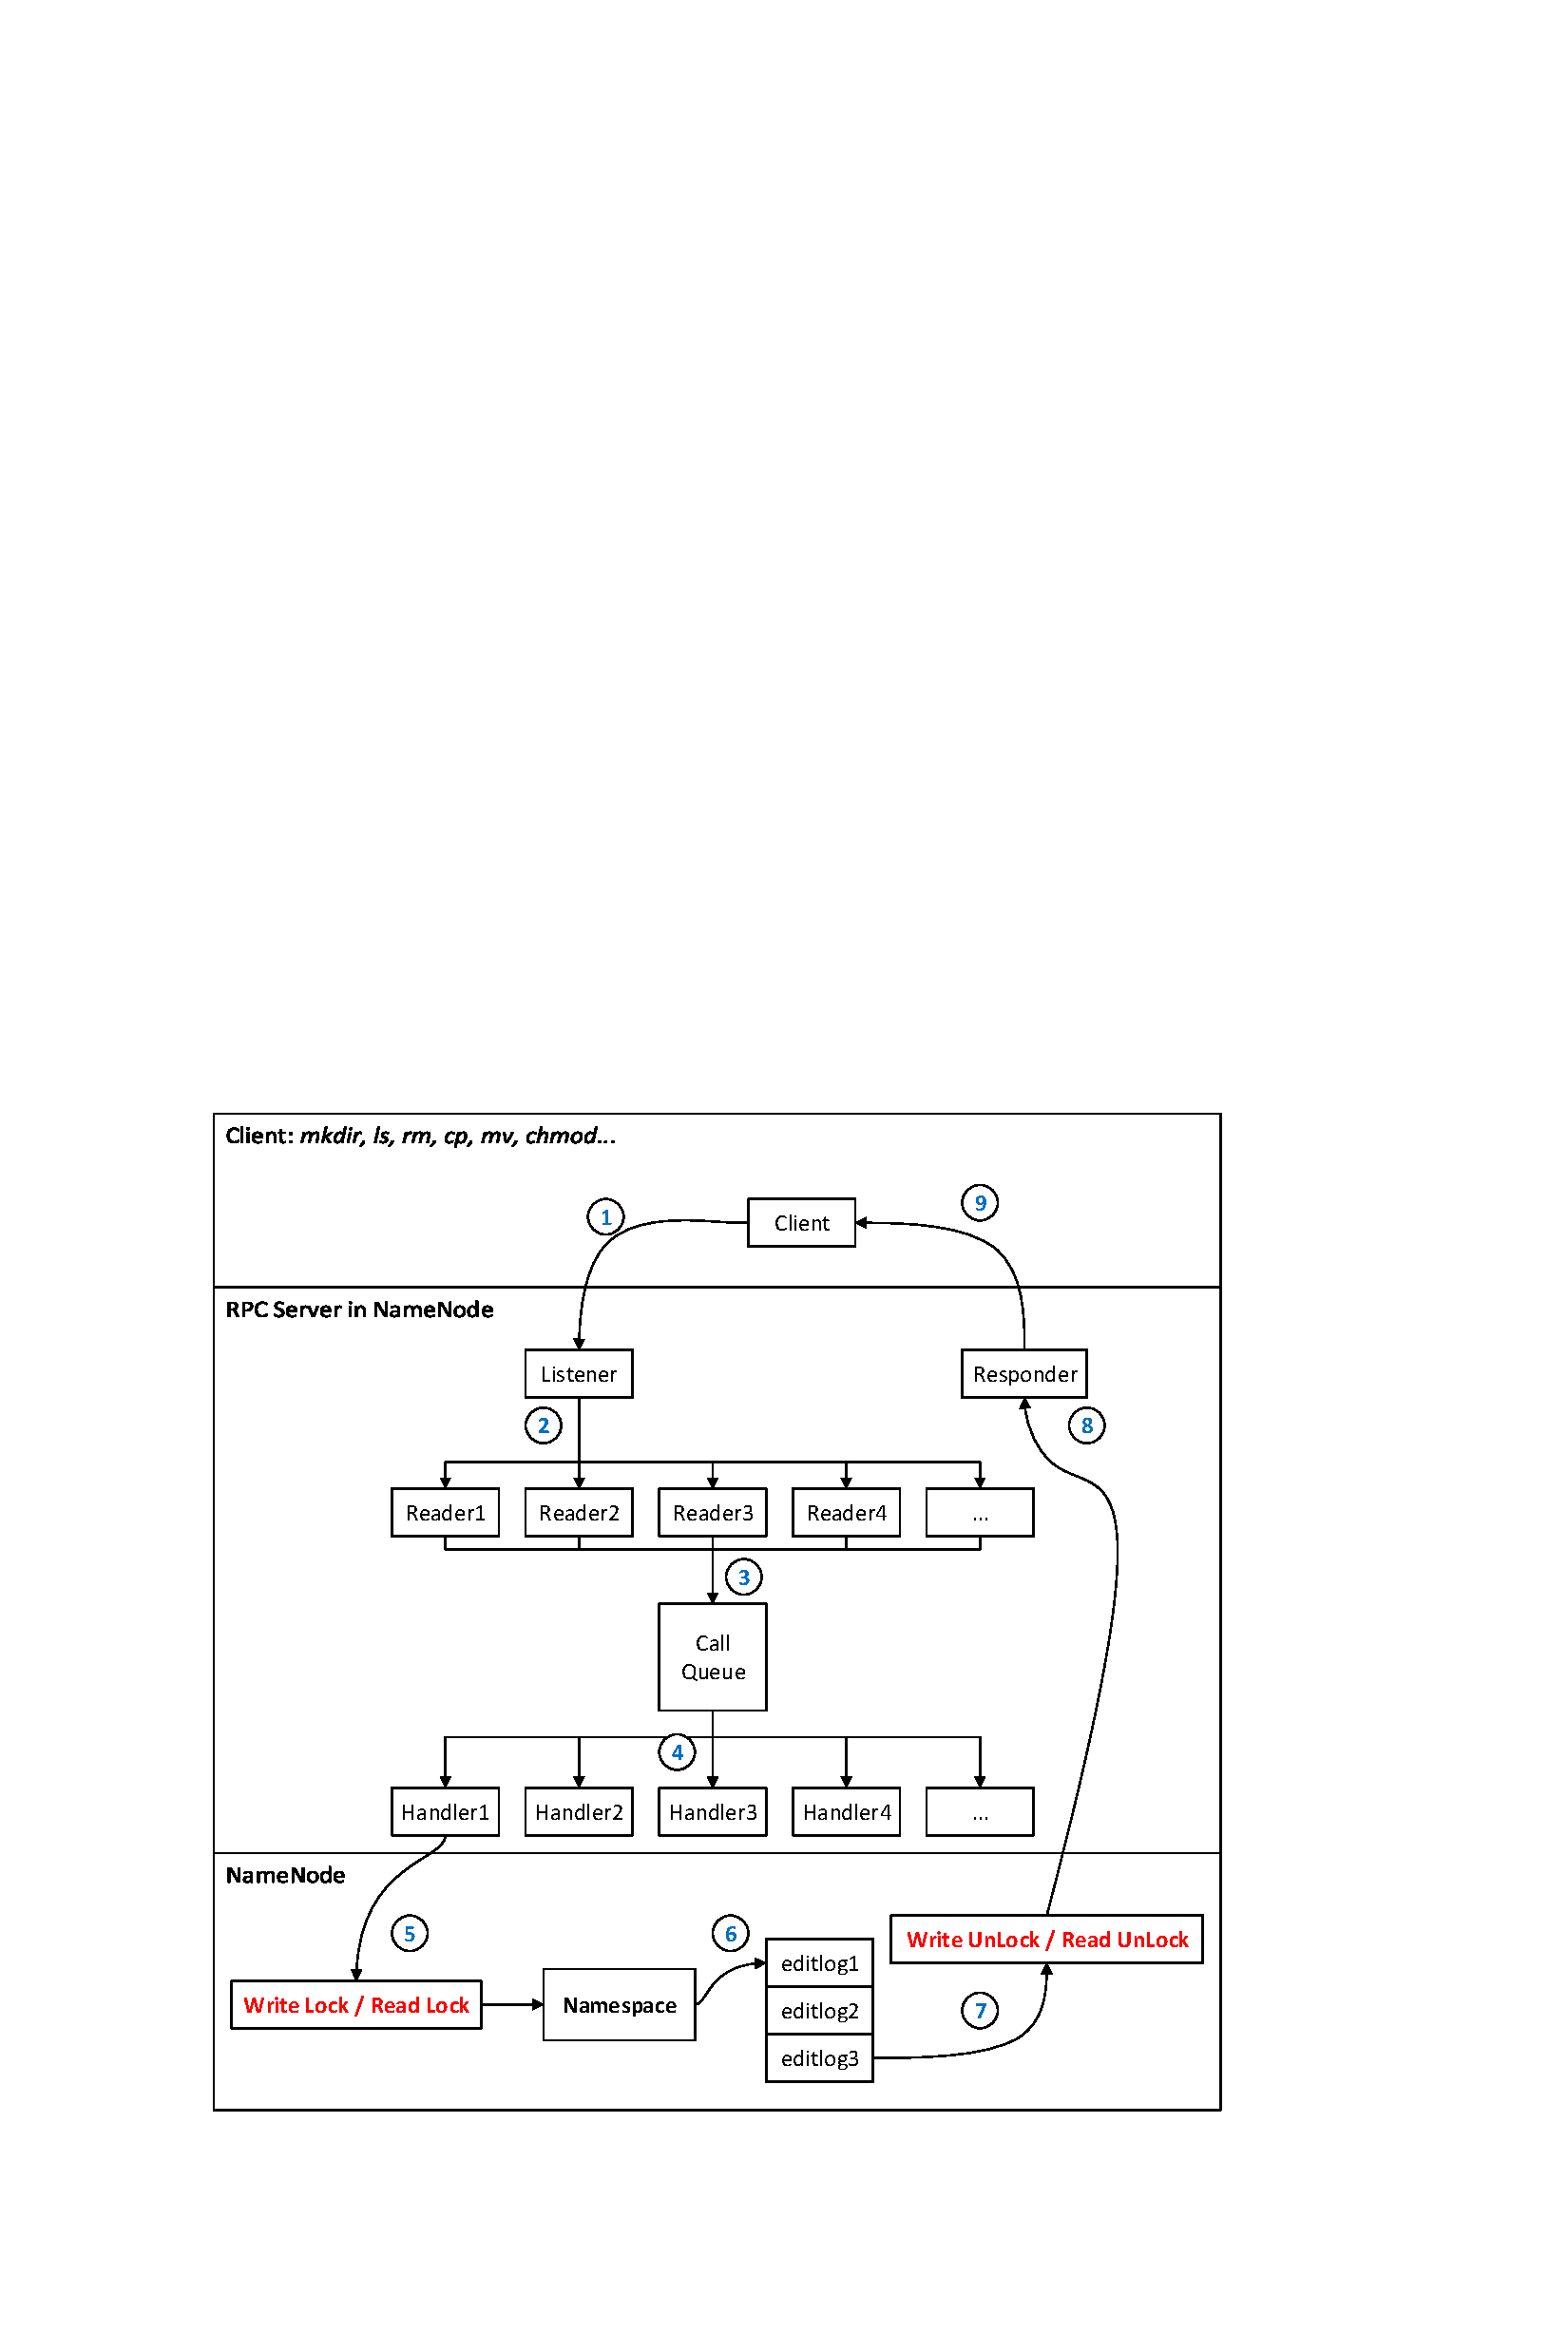
\includegraphics[scale=0.4]{figs/nnRPC.pdf}
		\end{figure}
\end{frame}

\subsection{Hop-HDFS Namespace Concurrency Control}
\begin{frame}
	\frametitle{HDFS Namespace Structure}
	\begin{columns}[c] % The "c" option specifies centered vertical alignment while the "t" option is used for top vertical alignment
	
	\column{.5\textwidth} % Left column and width
		\begin{figure}[h]
			\centering
			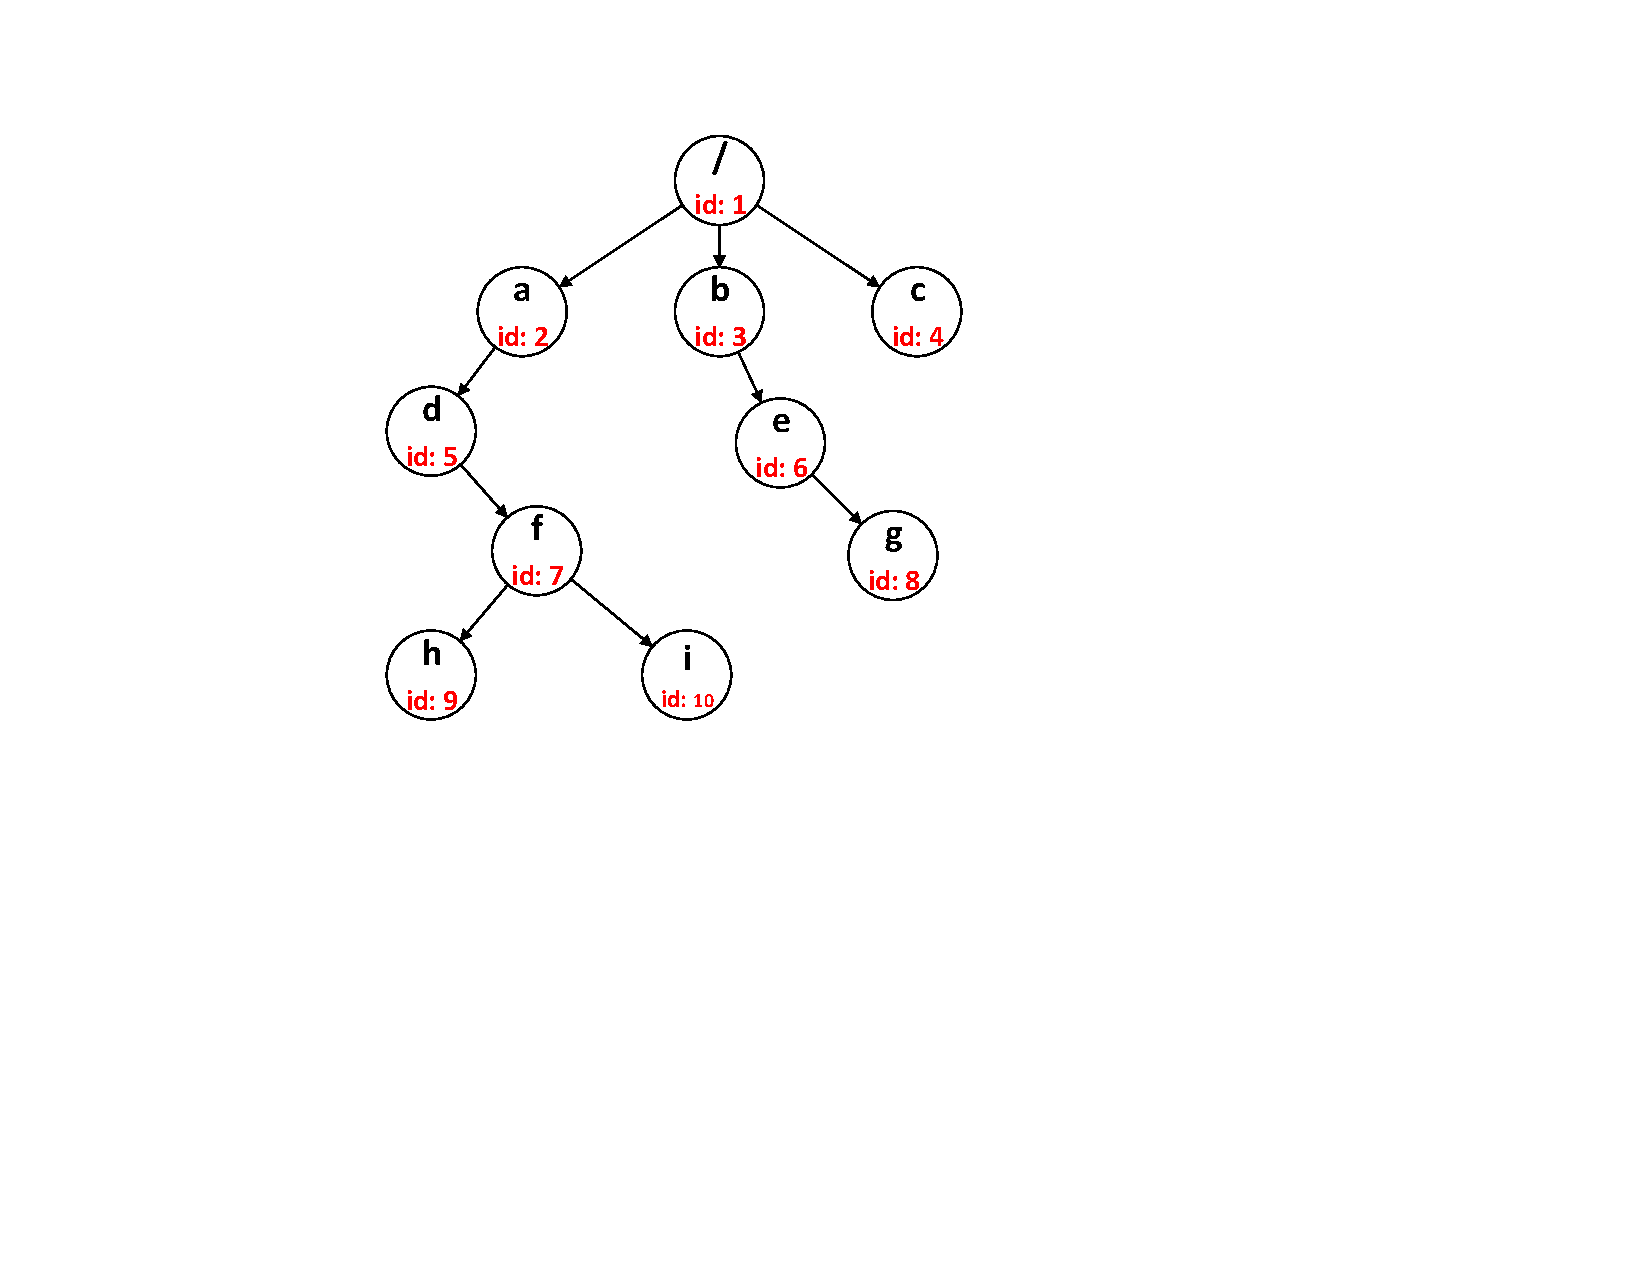
\includegraphics[scale=0.6]{figs/hoptree.pdf}
		\end{figure}
	
	\column{.5\textwidth} % Right column and width
	\begin{table}[h]
		\centering
		\begin{tabular}{|c|c|c|}
			\hline
			\textbf{id} & \textbf{parent\_id} & \textbf{name}\\ \hline
			1 & 0 & / \\ \hline
			2 & 1 & a \\ \hline
			3 & 1 & b \\ \hline
			4 & 1 & c \\ \hline
			5 & 2 & d \\ \hline
			6 & 3 & e \\ \hline
			7 & 5 & f \\ \hline
			8 & 6 & g \\ \hline
			9 & 7 & h \\ \hline
			10 & 7 & i \\ \hline
		\end{tabular}
	\end{table}
	
	\end{columns}
\end{frame}

\begin{frame}
\frametitle{Table}
\begin{table}
\begin{tabular}{l l l}
\toprule
\textbf{Treatments} & \textbf{Response 1} & \textbf{Response 2}\\
\midrule
Treatment 1 & 0.0003262 & 0.562 \\
Treatment 2 & 0.0015681 & 0.910 \\
Treatment 3 & 0.0009271 & 0.296 \\
\bottomrule
\end{tabular}
\caption{Table caption}
\end{table}
\end{frame}

%------------------------------------------------

\begin{frame}
\frametitle{Theorem}
\begin{theorem}[Mass--energy equivalence]
$E = mc^2$
\end{theorem}
\end{frame}

%------------------------------------------------

\begin{frame}[fragile] % Need to use the fragile option when verbatim is used in the slide
\frametitle{Verbatim}
\begin{example}[Theorem Slide Code]
\begin{verbatim}
\begin{frame}
\frametitle{Theorem}
\begin{theorem}[Mass--energy equivalence]
$E = mc^2$
\end{theorem}
\end{frame}\end{verbatim}
\end{example}
\end{frame}

%------------------------------------------------

\begin{frame}
\frametitle{Figure}
Uncomment the code on this slide to include your own image from the same directory as the template .TeX file.
%\begin{figure}
%\includegraphics[width=0.8\linewidth]{test}
%\end{figure}
\end{frame}

%------------------------------------------------

\begin{frame}[fragile] % Need to use the fragile option when verbatim is used in the slide
\frametitle{Citation}
An example of the \verb|\cite| command to cite within the presentation:\\~

%This statement requires citation \cite{p1}.
\end{frame}

%------------------------------------------------

\begin{frame}
\frametitle{References}
\footnotesize{
\begin{thebibliography}{99} % Beamer does not support BibTeX so references must be inserted manually as below
%\bibitem[Smith, 2012]{p1} John Smith (2012)
%\newblock Title of the publication
%\newblock \emph{Journal Name} 12(3), 45 -- 678.

\bibitem[\protect\citeauthoryear{Shvachko}{Shvachko}{2010}]{shvachko2010hdfs}
Shvachko, K.~V. (2010).
\newblock Hdfs scalability: The limits to growth.
\newblock {\em login\/}~{\em 35\/}(2), 6--16.

\end{thebibliography}
}
\end{frame}

%------------------------------------------------

\begin{frame}
\Huge{\centerline{Thank you.}}
\end{frame}

%----------------------------------------------------------------------------------------

\end{document} 